% build with lualatex plot.tex
\documentclass{programming}
\usepackage{auxhook}
%\usepackage{shellesc} % Needed with lualatex for tikz externalize
\usepackage{pgfplots}
\pgfplotsset{width=10cm,compat=1.9}

% We will externalize the figures
\usepgfplotslibrary{external}
\tikzexternalize

\newcommand{\joel}[1]{}

\begin{document}

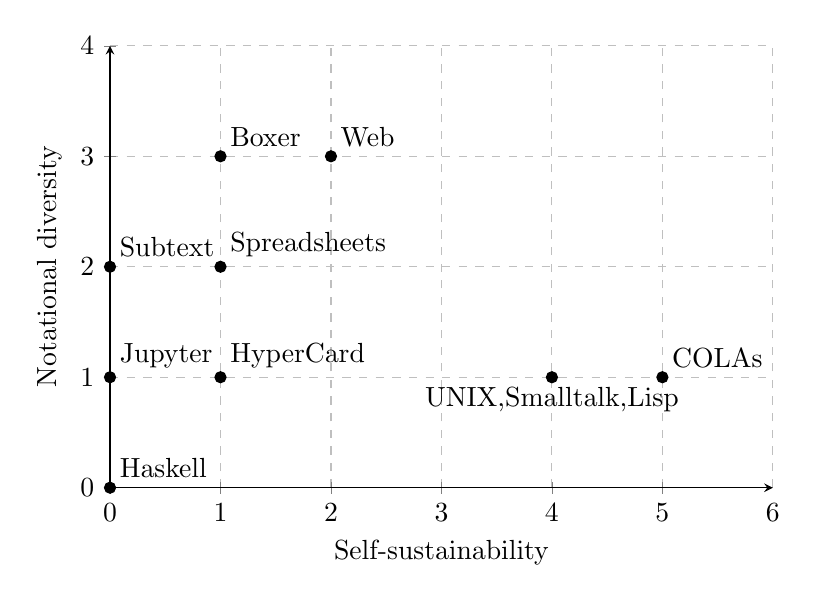
\begin{tikzpicture}
\begin{axis}[
    xlabel={Self-sustainability},
    ylabel={Notational diversity},
    xmin=0, xmax=6,
    ymin=0, ymax=4,
    %xtick={0,2,4,6,8,10},
    %ytick={0,2,4,6,8,10},
    axis lines=left,
    axis equal image,
    xmajorgrids=true,
    ymajorgrids=true,
    grid style=dashed,
    enlargelimits = false,
]
\addplot[
    scatter/classes={a={black}, b={blue}},
    scatter, mark=*, only marks, 
    scatter src=explicit symbolic,
    nodes near coords*={\Label},
    nodes near coords align=south west,
    visualization depends on={value \thisrow{label} \as \Label} %<- added value
] table [meta=class, row sep=crcr] {
    x y label class\\
    0 0 Haskell a\\
    0 1 Jupyter a\\
    1 2 Spreadsheets\\
    1 1 HyperCard a\\
    1 3 Boxer a\\
    2 3 Web a\\
    0 2 Subtext a\\
    5 1 COLAs a\\
};
\addplot[
    scatter/classes={a={black}, b={blue}},
    scatter, mark=*, only marks, 
    scatter src=explicit symbolic,
    nodes near coords*={\Label},
    nodes near coords align=north,
    visualization depends on={value \thisrow{label} \as \Label} %<- added value
] table [meta=class, row sep=crcr] {
    x y label class\\
    4 1 {UNIX,Smalltalk,Lisp} a\\
};
\end{axis}
\end{tikzpicture}

\end{document}
